\chapter{Methods}
\label{cha:Methods}

I want to disprove that the top-mentioned artists are mentioned for their style. This would mean that they are less used for their unique style but are added to prompts for other reasons.
When artists are not mentioned for their own unique style, the prompts in which they are mentioned should closely resemble other prompts in which they are not mentioned. Artists included for reasons other than their style should essentially be independent of the rest of a prompt.

There are many different ways of measuring the similarity between prompts. Since we focus on the analysis of styles in prompts, I will use direct references to styles to quantify the prompts. 


\section{Preprocessing}

The primary dataset contains 1.8 million prompts and metadata as mentioned in \ref{cha:Data}. The first step in the analysis is to detect the mentioned artists and styles in the prompts, the results are saved to separate files for the following steps.

\subsection{Detecting artists}


I use the large set of artist names and pseudonyms from the dataset \ref{cha:Artist Dataset}. Each prompt is analysed, the mentioned artists are extracted via an exact match of their full name or pseudonym. The amount of mentions of an artist across the entire dataset is counted and indicates the artist's popularity.

The first iteration of this preprocessing step did not include the analysis of pseudonyms. After analysing the resulting data, I found that many artists were mentioned by their real names and pseudonyms. I thus decided to include pseudonyms in the analysis.


\subsection{Detecting styles}


Similarly to the extraction of artists, the styles are extracted from the prompts via exact match. As a reference dataset of styles, I used the list \ref{cha:Styles Dataset} of 192 styles. 185 of the 192 styles were found in the prompts.




\section{Characterizing the artists}

To characterize the usage of an artist in the prompts, all prompts where an artist is mentioned are extracted. This group of prompts will be called the artist corpus.
The set of prompts that do not contain that artist are called the negative corpus. In all cases, the negative corpora are smaller than the artist corpus since no artist occurs in more than 50\% of the prompts.

The artist corpus and the respective negative corpus are computed for every artist. Artists without mentions in the dataset and artists that do not have any style mentions in their corpus are excluded from the analysis. The artist corpus and the corresponding negative corpus are used to compare the different artists.

The mentioned styles in the artist corpus and negative corpus are grouped and counted. The counts are normalized to proportions using the total amount of style mentions to enable comparisons between the two corpora.

\begin{figure}[h]
    \begin{center}
        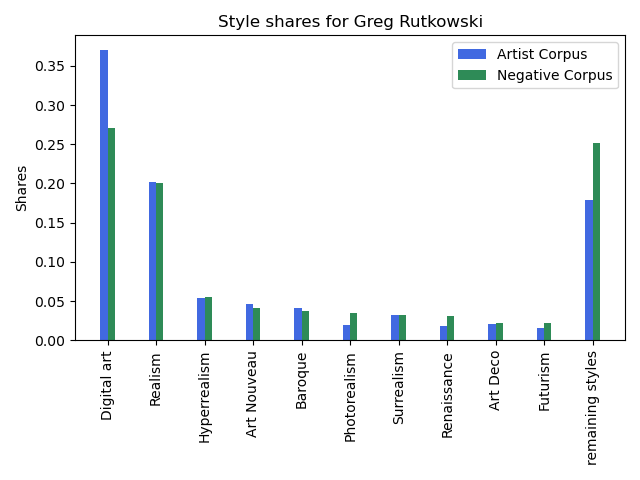
\includegraphics[height=7cm]{Bilder/style_proportions_example.png}\\[2.5ex]
    \end{center}
\caption{Example Style distribution for the 10 most popular styles and remaining styles}
\end{figure}


\section{Comparing Style distributions}

Artists with similar corpus and negative corpus have a smaller influence on the prompts they are used in. These artists are independent of the styles mentioned in the prompts.
I use the Bray-Curtis dissimilarity to evaluate the similarity between the two corpora. 
With these dissimilarity values, we can examine if there is a relation between the popularity of an artist and the artist's independence of the styles mentioned in the prompts.


\subsection{Bray-Curtis dissimilarity}

% stackexchange question
% https://stats.stackexchange.com/questions/609149/similarity-measure-for-two-discrete-distributions-a-group-of-proportions

% Comparison metrics is scaled in 0 to 1....
 %Soerensen-Dice coefficient
% https://en.wikipedia.org/wiki/S%C3%B8rensen%E2%80%93Dice_coefficient

%DSC =Dice similarity coefficient

%\[ DSC = \frac{2|X \cap Y|}{|X| + |Y|}\]

%Since \(|X|\) and \(|Y|\) are always one, we can simplify the formula to:

%\[ DSC = |X \cap Y|\]

% It is easier to use and reference the Bray Curtis dissimilarity

For comparing the style distributions, I will use the Bray-Curtis dissimilarity. It comes from Biology and quantifies the compositional dissimilarity between two sites, based on counts. In this case, we are comparing the style distributions of the artist corpus \(i\) with the negative corpus \(j\). The dissimilarity value is 0 for identical distributions and 1 for distributions without common elements. It is defined as:

\[ BC_{ij} = 1 - \frac{2C_{ij}}{S_i + S_j}\]

Since we express the style mentions as proportions, the sizes \(S_i\) and \(S_j\) are always one. The forluma is simplified to:

\[ BC_{ij} = 1 - C_{ij} \]


\(C_{ij}\) is the sum of the lesser values for styles in common between the compared prompts:

\[ C_{ij} = \sum_{s \in Styles} min(i_s,j_s)\]

Figure \ref{fig:dissimilarity_calculation_example} shows the calculation of a dissimilarity value. The red bars represent the shares \(min(i_s,j_s)\), that the style distributions of the artist corpus and negative corpus have in common. The summation of all the red bars equates to \(C_{ij}\). 

\begin{figure}[h]
    \begin{center}
        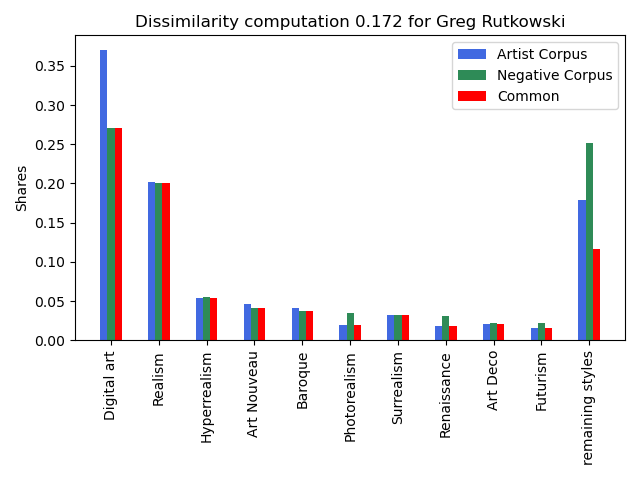
\includegraphics[height=7cm]{Bilder/dissimilarity_calculation_example.png}\\[2.5ex]
    \end{center}
\caption{Example Dissimilarity calculation}
\label{fig:dissimilarity_calculation_example}
\end{figure}



\subsection{Evaluating the observed dissimilarity}

The observed dissimilarity values will be analysed with Spearman's rank correlation coefficient. This correlation coefficient is chosen since it is appropriate for comparing two ranked variables and does not require the variables to satisfy conditions such as being normally distributed. In this case, the coefficient indicates whether the artist's popularity rank correlates with the style distributions' dissimilarity. The coefficient produces an \(r_s\) value between -1 and 1, where 1 indicates a perfect positive correlation, 0 indicates no correlation and -1 indicates a perfect negative correlation.

To check the significance of the correlation, we will use the \(p\) value of the Spearman's rank correlation coefficient. This \(p\) value is for a hypothesis test, where the null hypothesis states that the two variables are not correlated.

% The observed dissimilarity values will be visualized as well.




% if the p value is small, we have to reject the null hypothesis
